\hypertarget{4}{}

\chapter{Extracting Phenotype-Gene Relations}

\rhead{Extracting Phenotype-Gene Relations}
\lhead{Chapter 4}

\vspace{-1.6cm}

% Gray Line
\begingroup
\color{gray}
\par\noindent\rule{\textwidth}{0.4pt}
\endgroup

\noindent{Human phenotype-gene relations described in biomedical literature can be used to annotate specialized databases and provide a deeper understanding of the origin of some phenotypic abnormalities and their associated diseases. Most Relation Extraction (RE) approaches use supervised machine learning methods that require annotated data sets. The work developed in Chapter \hyperlink{3}{3} successfully tackles the lack of data sets with the creation of the PGR corpus, using a distant supervision approach to extract the human phenotype-gene relations. However, biomedical RE machine learning systems are not prepared to deal with the specifics of human phenotype and gene entities, and their relations. This chapter proposes two different learning approaches (\textbf{Distantly Supervised Multi-instance Learning} and \textbf{Deep Learning}) for human phenotype-gene RE. These methods were developed based on existing biomedical RE systems that were modified to accommodate human phenotype-gene RE:}

\begin{itemize}
   \item \textbf{IBRel} \citep{10.1371/journal.pone.0171929} is a biomedical RE system, based on distantly supervised multi-instance learning, developed to extract miRNA-gene relations in the text. This system uses the TransmiR database \citep{10.1093/nar/gkp803} as a knowledge base for gold standard miRNA-gene relations. The system combines distant supervision with a multi-instance learning approach, based on the sparse multi-instance learning (sMIL) algorithm \citep{Bunescu:2007:MIL:1273496.1273510}, to filter negative candidate pairs.
   \item \textbf{BO-LSTM} \citep{BOLSTM} is the first biomedical RE system to incorporate semantic and ancestry information from biomedical ontologies along with deep learning techniques. BO-LSTM is a system that was developed to detect and classify drug-drug interactions in text. The system represents each entity as the sequence of its ancestors in an ontology, using the Chemical Entities of Biological Interest (ChEBI) ontology \citep{CHEBI}. In addition to ontologies, it uses word embeddings and WordNet \citep{WORDNET} data representations to perform biomedical RE.
\end{itemize}

This chapter will present a brief overview of the general methods used to create the IBRel and the BO-LSTM classifiers, and a detailed description of the necessary system adjustments to accommodate human phenotype-gene RE. These system modules, dedicated to human phenotype-gene RE, will be evaluated using the PGR corpus developed in Chapter \hyperlink{3}{3}. To further discuss the benefits of each approach, it is relevant to employ other RE approaches, namely, a co-occurrence (or all-true) baseline method, the state-of-the-art BioBERT application \citep{BIOBERT}, and a bootstrap theoretical approach that leverages of both developed modules, also using the PGR corpus. Finally, the chapter will end with the presentation of the results of all the implementations and a comprehensive discussion of the benefits and downsides of each approach.


% ------------------------------> METHODS

\section{Methods}

The main goal of all of the models described in this chapter is to extract relations from unstructured or highly heterogeneous text. However, each system expects different data format inputs (instances) and uses resources of distinct external sources of knowledge plus the training data to build them. This section will provide an overview of these differences, and the necessary steps to successfully perform human phenotype-gene RE using these learning methods.


% ----------------> DISTANTLY SUPERVISED MULTI-INSTANCE LEARNING MODULE

\hypertarget{4.1.1}{\subsection{Distantly Supervised Multi-instance Learning Module}}

The resources needed to perform distantly supervised multi-instance learning (the input text and a knowledge base) were already presented in Chapter \hyperlink{3}{3}. The knowledge base for the application of this method was also the HPO gold standard relations knowledge base that links phenotypic abnormalities to genes, with the added synonyms for the gene entities. Therefore, this section will focus on the \textit{bag-of-instances} representations, the model itself, and the necessary changes needed to perform human phenotype-gene RE. Figure \ref{figure:ibrel_workflow} shows the IBRel system general workflow, and a model simplification in bold.

The input data is used to generate instances to be classified by the model. Each instance represents a candidate pair of entities and consists of multiple relevant data representations besides the entities offsets. For example, using word context windows (of sizes 1, 3, and 5), each word, in each sentence fragment that encompasses a candidate relation, goes through lemmatization and part-of-speech (POS) tagging. Then, these instances are converted into \textit{bag-of-instances} representations, using the scikit-learn library \citep{scikit-learn}.

\begin{figure}[ht]
\captionsetup{font=small}
\centering
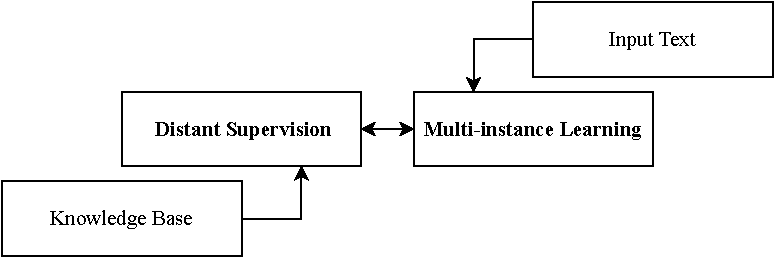
\includegraphics[width=13cm]{images/ibrel_workflow.pdf}
\fontsize{9}{10.8}\caption[IBRel Workflow]{IBRel workflow. The input text corresponds to sentences retrieved from PubMed abstracts, and the knowledge base corresponds to the HPO gold standard relations knowledge base. The double arrow represents a dependency between the multi-instance learning step and the distant supervision step. Each \textit{bag} created by the multi-instance learning step is labeled positive if a pair exists in the reference knowledge base, and negative otherwise.}
\label{figure:ibrel_workflow}
\end{figure}

% ------> BAG-OF-INSTANCES REPRESENTATIONS AND MODEL 

\subsubsection{\textit{Bag-of-Instances} Representations and Model}

Multi-instance learning is a particular case of a supervised machine learning method since it uses a training-set composed of labeled \textit{bags} instead of labeled instances. The multi-instance learning approach performed is based on the sMIL algorithm. The sMIL algorithm assumes that the data is sparse, implicating that for each \textit{bag} only a few candidate pairs are positive. The general assumption is that if two entities preserve a relation in a knowledge base, at least one sentence that mentions the entity pair expresses the relation \citep{Surdeanu:2012:MML:2390948.2391003}. Thus, it is necessary to decide how to represent human phenotype-gene relations in the form of \textit{bags}. 

In this model, each \textit{bag} is an instance that can contain multiple entries corresponding to the same relation candidate, for the entire corpus. Figure \ref{figure:ibrel_bags} presents an example sentence retrieved from the PGR corpus, with five entity annotations. Taking into account that entity E1 and entity E5 are the same, in this sentence, it is possible to extract four unique candidate pairs, that correspond to four different \textit{bags} with the distinct text mentions. A \textit{bag} is labeled as positive (label 1) if the candidate pair exists in the reference knowledge base, and negative (label 0) if the candidate pair does not correspond to an entry in the knowledge base.

\begin{figure}[ht]
\captionsetup{font=small}
\centering
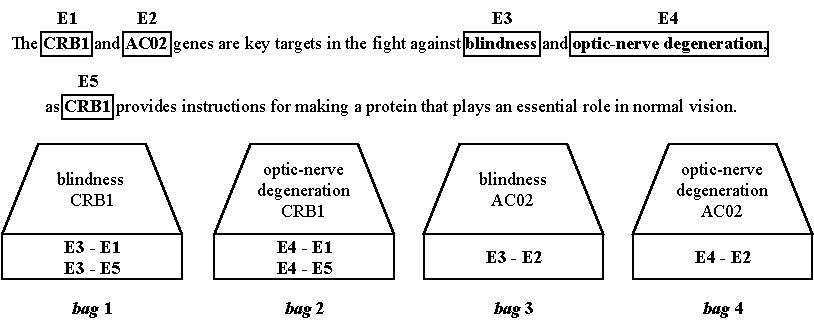
\includegraphics[width=15cm]{images/ibrel_bags.pdf}
\fontsize{9}{10.8}\caption[Multi-instance Learning \textit{Bags}]{Multi-instance learning \textit{bags}. Each \textit{bag} represents one instance, a representation of a candidate human phenotype-gene relation, for the corpus. The \textit{bags} 1 and 4 are positive (labeled 1), and the \textit{bags} 2 and 3 are negative (labeled 0).}
\label{figure:ibrel_bags}
\end{figure}

After creating the \textit{bags}, the sMIL algorithm was used to generate the classification model, using the miSVM package\footnote{\url{https://github.com/garydoranjr/misvm}}, with the default values. 

The original IBRel system source code was in Python 2.7. For the new human phenotype-gene RE model the source code was updated to Python 3.6\footnote{\url{https://github.com/lasigeBioTM/IBRel/tree/IBRel_Python3.6}}. Most of the original packages were incompatible with this new version of the system but there were updated versions available. One of the most relevant packages for this system is the miSVM that did not have an updated version. Therefore, it was necessary to develop a Python 3 miSVM compatible version to apply to the model. 

% ----------------> DEEP LEARNING MODULE

\hypertarget{4.1.2}{\subsection{Deep Learning Module}}

This section describes the BO-LSTM model with an emphasis on the modifications to allow human phenotype-gene RE integration. Figure \ref{figure:bo_lstm_architecture} shows a simplification of the overall model architecture. 

\begin{figure}[ht]
\captionsetup{font=small}
\centering
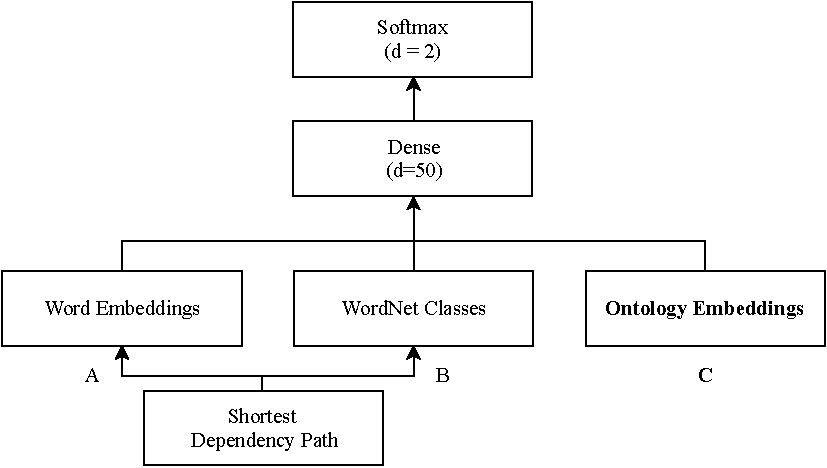
\includegraphics[width=14cm]{images/bo_lstm_architecture.pdf}
\fontsize{9}{10.8}\caption[BO-LSTM Model Architecture Simplification]{BO-LSTM model architecture simplification. \textbf{(A)}, \textbf{(B)} and \textbf{(C)} represent the three primary data information layers that are fed to the model. \textit{d} is the dimensionality of each embedding layer, \textbf{(A)} corresponds to the Word Embeddings, \textbf{(B)} to the WordNet Channel and \textbf{(C)} the Ontology Embeddings.}
\label{figure:bo_lstm_architecture}
\end{figure}


% ------> DATA REPRESENTATIONS

\hypertarget{4.1.2.1}{\subsubsection{Data Representations}}

The BO-LSTM model uses a combination of different language and entity related data representations, that feed individual channels creating a multichannel architecture. The input data is used to generate instances to be classified by the model. Each instance corresponds to a candidate pair of entities in a sentence. To each instance, the model is going to assign a positive or negative class. In this case study, a positive class corresponds to an identified relation between a human phenotype and a gene entity, where the nature of this relation is always of \textit{causality}, and a negative class implies no relation between the different entities.

An instance should condense all relevant information to classify a candidate pair. To create an instance the BO-LSTM model relies on three primary data information layers (Figure \ref{figure:bo_lstm_architecture}). After sentence tokenization, these layers are:

\begin{itemize}
   \item \textbf{Shortest Dependency Path (SDP)} between the entities of the candidate pair. For instance, in the sentence \textit{The \textbf{CRB1} gene is a key target in the fight against \textbf{blindness}}, the shortest path between the entities would be \textbf{CRB1} - gene - is - target - in - fight - against - \textbf{blindness}, using the spaCy software library\footnote{\url{https://spacy.io/}}. Every word is replaced by a generic string to minimize the impact of specific words in the model. The model uses pre-trained word embeddings vectors trained on abstracts and full documents from PubMed (more than 29 million) \citep{Pyysalo:2013b}, using the Word2Vec algorithm \citep{Mikolov:2013:DRW:2999792.2999959}. These vectors are more relevant for biomedical tasks than vectors trained on a generic corpus.
   
   \item \textbf{WordNet Classes}, using the tool developed by \cite{Ciaramita:2006:BSD:1610075.1610158}, matches each element in the SDP to a WordNet hypernym class. For instance, using the previous sentence, it would be \textbf{CRB1}\textsubscript{noun.e1} - gene\textsubscript{noun} - is\textsubscript{verb} - target\textsubscript{noun} - in\textsubscript{adverb} - fight\textsubscript{noun} - 0 - blindness\textsubscript{noun.e2}.
   
   \item \textbf{Ontology Embeddings} represents the relations between the ancestors for each ontology concept corresponding to an entity (Figure \ref{figure:model_ds}).
\end{itemize}

The model assumes that the input data already has the offsets of the relevant entities identified and their respective concept ID, the Named-Entity Recognition and Linking tasks. However, while human phenotype entities identifiers already corresponded to an ontology concept ID (Human Phenotype Ontology (HPO) \citep{HPO}), gene entities had only a National Center for Biotechnology Information (NCBI) identifier\footnote{\url{https://www.ncbi.nlm.nih.gov/}}. Genes have several designated ontologies, for example the Gene Ontology \citep{GO} that describes gene properties/attributes. The Gene Ontology provides a computational representation of our current scientific knowledge about the functions of genes and it is widely used to support scientific research.

The solution to overcome this problem was to match each gene to their most representative GO concept within the \textit{biological process} category (sub-ontology). Each gene has a corresponding set of GO terms inferred from different sources and with different degrees of confidence. NCBI provides a list\footnote{\url{https://ftp.ncbi.nlm.nih.gov/gene/DATA/}} of genes to GO relations and their evidence codes. There are twenty-six different evidence codes, that fall into six general categories: experimental evidence codes (\textbf{EXP}, \textbf{IDA}, \textbf{IPI}, \textbf{IMP}, \textbf{IGI}, \textbf{IEP}, \textbf{HTP}, \textbf{HDA}, \textbf{HMP}, \textbf{HGI}, and \textbf{HEP}), phylogenetically-inferred annotations (\textbf{IBA}, \textbf{IBD}, \textbf{IKR}, and \textbf{IRD}), computational analysis evidence codes (\textbf{ISS}, \textbf{ISO}, \textbf{ISA}, \textbf{ISM}, \textbf{IGC}, and \textbf{RCA}), author statement evidence codes (\textbf{TAS}, and \textbf{NAS}), curator statement evidence codes (\textbf{IC}, and \textbf{ND}), and electronic annotation evidence code (\textbf{IEA}) (Table \ref{table:evidence}). To match the gene to their most representative GO term the priority was given to concepts inferred from experiments, for having a more sustained background and usually be more descriptive (Example \hyperlink{ex4.1}{4.1}). For tie-breaking, if we have several GO terms inferred from experiments, the choice is the one term that is the most specific with the longer ancestry line.

\begin{table}[!ht]
\renewcommand\arraystretch{1.2}
\small
\captionsetup{font=small}
\caption[Gene Ontology Evidence Codes]{Gene Ontology (GO) evidence codes.} 
\centering
\taburulecolor{black}
\newcolumntype{C}{ >{\centering\arraybackslash} m{8.5cm} }
\newcolumntype{D}{ >{\centering\arraybackslash} m{4cm} }
\begin{tabular}{|D|C|}

\hline
\textbf{Category} & \textbf{Evidence Codes} \\
\hline\hline
\multirow{11}{*}{\textbf{Experimental}} & Inferred from Experiment (EXP) \\
\cline{2-2}
& Inferred from Direct Assay (IDA) \\
\cline{2-2}
& Inferred from Physical Interaction (IPI) \\
\cline{2-2}
& Inferred from Mutant Phenotype (IMP) \\
\cline{2-2}
& Inferred from Genetic Interaction (IGI) \\
\cline{2-2}
& Inferred from Expression Pattern (IEP) \\
\cline{2-2}
& Inferred from High Throughput Experiment (HTP) \\
\cline{2-2}
& Inferred from High Throughput Direct Assay (HDA) \\
\cline{2-2}
& Inferred from High Throughput Mutant Phenotype (HMP) \\
\cline{2-2}
& Inferred from High Throughput Genetic Interaction (HGI) \\
\cline{2-2}
& Inferred from High Throughput Expression Pattern (HEP) \\
\hline\hline
\multirow{4}{*}{\textbf{Phylogenetically-inferred}} & Inferred from Biological aspect of Ancestor (IBA) \\
\cline{2-2}
& Inferred from Biological aspect of Descendant (IBD) \\
\cline{2-2}
& Inferred from Key Residues (IKR) \\
\cline{2-2}
& Inferred from Rapid Divergence (IRD) \\
\hline\hline
\multirow{6}{*}{\textbf{Computational Analysis}} & Inferred from Sequence or structural Similarity (ISS) \\
\cline{2-2}
& Inferred from Sequence Orthology (ISO) \\
\cline{2-2}
& Inferred from Sequence Alignment (ISA) \\
\cline{2-2}
& Inferred from Sequence Model (ISM) \\
\cline{2-2}
& Inferred from Genomic Context (IGC) \\
\cline{2-2}
& Inferred from Reviewed Computational Analysis (RCA) \\
\hline\hline
\multirow{2}{*}{\textbf{Author Statement}} & Traceable Author Statement (TAS) \\
\cline{2-2}
& Non-traceable Author Statement (NAS) \\
\hline\hline
\multirow{2}{*}{\textbf{Curator Statement}} & Inferred by Curator (IC) \\
\cline{2-2}
& No biological Data available (ND) \\
\hline\hline
\textbf{Electronic Annotation} & Inferred from Electronic Annotation (IEA) \\
\hline

\end{tabular}
\label{table:evidence}
\end{table}

\bigskip

% EXAMPLE 4.1

\hypertarget{ex4.1}{\textbf{Example 4.1}} Selection of the most representative GO term for the CRB1 gene, organized by priority order of the evidence code.

\begin{itemize}

\item\textbf{Gene:} \textit{CRB1}
\item\textbf{Gene NCBI Identifier:} 23418
\item\textbf{Biological Process Annotations:}

\begin{itemize}
\item GO:0007009 - IEA - plasma membrane organization \textbf{(4th)}
\item \textbf{GO:0007157 - EXP - heterophilic cell-cell adhesion via plasma membrane cell adhesion molecules (1st)}
\item GO:0007163 - TAS - establishment or maintenance of cell polarity \textbf{(3rd)}
\item GO:0045197 - IBA - establishment or maintenance of epithelial cell apical/basal polarity \textbf{(2nd)}
\end{itemize}

\end{itemize}

% END EXAMPLE 4.1


% ------> MODEL 

\subsubsection{Model}

The most relevant part of this work is the implementation of the ontology embeddings in the model. An ontology describes a formal definition of concepts related to a specific subject and can be represented by a tuple $<C, R>$, where $C$ represents the set of concepts in an ontology and $R$ the set of relations between the concepts of the same ontology. The type of ontology relations considered were subsumption relations, \textbf{is-a} due to its transitive aspect. For instance, if we have $(c_1, c_2) \in R$, and $(c_2, c_3) \in R$, we assume that $(c_1, c_3)$ is a valid relation within the ontology. The ancestors of each concept $c$ are given by:

\begin{equation}
\small
Anc(c) = a : (c, a) \in T
\label{equation:ancestors}
\end{equation}

where $T$ is the transitive closure of $R$. A relation between different ontology concepts can be represented by $(p_1, g_1)$, where $p_1 \in P$ and $P$ represents the set of concepts in the HPO, and $g_1 \in G$ and $G$ represents the set of concepts in the Gene Ontology. For instance, if we have $(p_2, g_2) \in RA$, where $RA$ is the set of relations between ancestors, and $p_2\,\textbf{is-a}\,p_1$, and $g_2\,\textbf{is-a}\,g_1$, then we can assume that $(p_1, g_1)$ is a valid relation. The concatenation of the relations between the ancestors of concepts $p_2$ and $g_2$ can be defined using:

\begin{equation}
\small
ConcRA(p_2, g_2) = Anc(p_2) \Join Anc(g_2)
\label{equation:cancestors}
\end{equation}

Figure \ref{figure:model_ds} shows an overview of a representation for a candidate pair based on the ancestry of its elements, using the most representative GO term as shown in Example \hyperlink{ex4.1}{4.1}. 

\begin{figure}[ht]
\captionsetup{font=small}
\centering
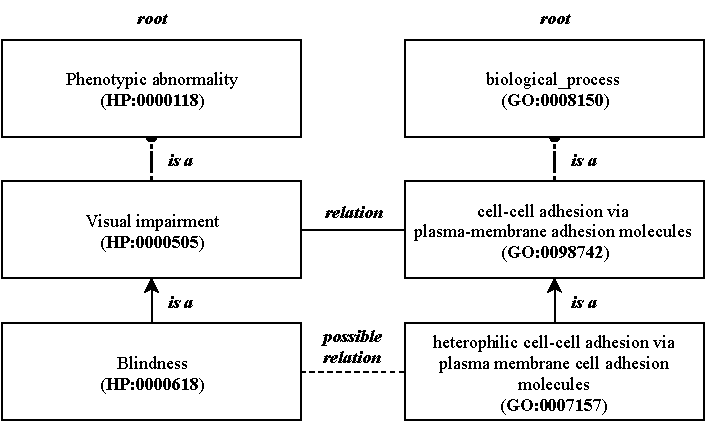
\includegraphics[width=13cm]{images/model_ds.pdf}
\fontsize{9}{10.8}\caption[BO-LSTM Ontology Embedding Illustration]{BO-LSTM ontology embedding illustration based on the HPO and the Gene Ontology, for the candidate relation between the human phenotype \textit{blindness} and the gene \textit{CRB1} (represented by the GO term \textit{heterophilic cell-cell adhesion via plasma membrane cell adhesion molecules})}
\label{figure:model_ds}
\end{figure}

Figure \ref{figure:lstm_detailed} presents the detailed workflow of the Ontology Embeddings in Figure \ref{figure:bo_lstm_architecture}. Each concatenation of relations between ancestors corresponds to one-hot vector $v_c$, a vector of zeros except for the position that corresponds to the ID of the concepts. An embedding matrix $M \in \mathbb{R}^{D \times C}$ transforms these sparse vectors into dense vectors, where $D$ is the dimensionality of the embedding layer and $C$ is the number of concepts of the ontologies. Then, the output of the embedding layer is given by:

\begin{equation}
\small
f(c) = M \cdot v_c
\label{equation:ontologyembedding}
\end{equation}

Formerly, the ontology embedding layer, with a dimensionality of 50, initializes its values randomly so that they could later be tuned, through back-propagation. This size was the one that performed the best after testing with the sizes 50, 100, and 150, as suggest by \cite{xu-etal-2015-classifying}. Then, the sequence of vectors representing the relations between the ancestors of the terms is fed into the LSTM layer, showed in detail in Figure \ref{figure:lstm_detailed}. Finally, the system uses a max pool layer, which is fed into a dense layer through a sigmoid activation function, and a softmax layer outputs the probability for each class.

\begin{figure}[ht]
\captionsetup{font=small}
\centering
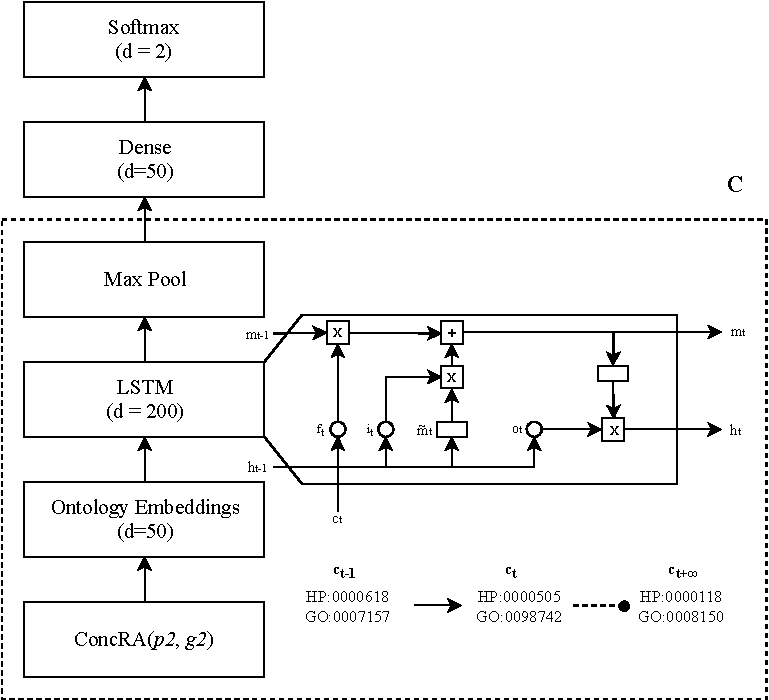
\includegraphics[width=13cm]{images/lstm_detailed.pdf}
\fontsize{9}{10.8}\caption[Ontology Embeddings Workflow]{Ontology embedding workflow, using the sequence in Figure \ref{figure:model_ds} as an example. $\circ$ refers to sigmoid function, $\rectangle$ to tanh, $x$ to element-wise multiplication, and $+$ to element-wise addition. $h$ is the hidden unit, $\tilde{m}$ the candidate memory cell, $m$ a memory cell, $i$ the input gate, $f$ the forget gate, and $o$ the output gate.}
\label{figure:lstm_detailed}
\end{figure}

Deep learning models map a set of inputs to a set of outputs from the training data. It is not feasible to calculate the perfect weights for a neural network, because it is not a linear problem. Thus, the issue of learning assumes the form of an optimization problem. To approach this optimization problem, we use different optimization algorithms to try to enhance our predictions. In this work, the model was trained using a stochastic gradient descent optimization algorithm where weights were updated using the back-propagation of error algorithm. At each iteration, the model with a given set of weights creates predictions and computes the error for those predictions. The optimization algorithm seeks to alter the weights to reduce that error in the next evaluation. The relevant configurations of this model are:

\begin{itemize}
   \item \textbf{Mini-batch Gradient Descent Optimization Algorithm}: RMSprop.
   \item \textbf{Learning Rate}: 0.001 (default value for RMSprop).  
   \item \textbf{Loss Function}: Categorical Crossentropy.
   \item \textbf{Dropout Rate}: 0.500 (every layer except the penultimate and output layers).
\end{itemize}

The dropout strategy adopted \citep{journals/corr/abs-1207-0580} reduced the overfitting on the trained embeddings and weights. 

% ------------------------------> EVALUATION

\section{Evaluation}

The corpus used to evaluate each module was the PGR corpus, described in Chapter \hyperlink{3}{3}. The measures used to evaluate the performance of the RE modules were precision, recall, and F-measure.

To further assess the quality of the developed implementations, it was relevant to employ other RE approaches, namely a co-occurrence baseline method, the state-of-the-art application BioBERT, and a bootstrap theoretical approach that leverages both developed modules. These approaches were also evaluated using the PGR corpus. 

% ----------------> CO-OCCURRENCE BASELINE METHOD

\subsection{Co-occurrence Baseline Method}

The applied co-occurrence approach consists of considering every human phenotype-gene pair in the same sentence as positive. This approach produces a high number of false positives and results in a recall of 1. For even distributions of positive/negative pairs, and specifically for abstracts, the co-occurrence method can achieve, for some data sets, almost state-of-the-art results \citep{10.1093/database/baz030}.

% ----------------> BIOBERT APPLICATION

\subsection{BioBERT Application}

The BioBERT system is a new pre-trained biomedical language representation model for biomedical text mining based on the BERT \citep{BERT} architecture. This system, trained on large-scale biomedical corpora, can perform diverse biomedical text mining tasks, namely Named-Entity Recognition (NER), RE and Question Answering (QA). The novelty of the architecture is that these systems, BioBERT and BERT, are designed to pre-train deep bidirectional representations by jointly conditioning on both left and right context in all layers. This feature allows easy adaption to several tasks without loss in performance.

The PGR corpus was trained and tested using the available pre-trained weights of the BioBERT model. It was necessary to anonymize the test-set entities, using the pre-defined tags \textit{@GENE} for gene entities and \textit{@DISEASE} for human phenotype entities, for being the tags available closest to the case study of this thesis (human phenotype-gene relations).

% ----------------> BOOTSTRAP APPROACH (THEORETICAL)

\subsection{Bootstrap Approach (Theoretical)}

The bootstrap approach implemented combines the results obtained from the first system (Distantly Supervised Multi-instance Learning Module, Section \hyperlink{4.1.1}{4.1.1}) with the second system (Deep Learning Module, Section \hyperlink{4.1.2}{4.1.2}). Thus, for each candidate pair, if the classifiers disagree on the classification, and one of them classifies the candidate pair with the correct label, that would be the chosen label. Since this approach requires knowledge of the true labels of the test-set, it cannot be used as a classifier for unlabeled data. This approach is relevant because it allows us to know where each system fails, i.e., both systems classify the same sentence in the same way (true positive, false negative, false positive, or true negative) or if their classification differs, and how much it differs, and why.


% ------------------------------> RESULTS AND DISCUSSION

\section{Results and Discussion}

Each implementation was evaluated using the PGR corpus, developed in Chapter \hyperlink{3}{3}. However, before presenting the final results it is necessary to mention some evaluation limitations. It is not possible to dissociate this evaluation from the quality of the NER, Named-Entity Linking (NEL) and RE tasks performed in the previous chapter. If some entities were poorly identified, not identified at all, or not linked to the right identifier, then this will reflect on the performance of each different implementation, when using the PGR corpus. Also, the RE task was performed using a distant supervision approach resorting to a gold standard knowledge base of relations that is still evolving, growing, and therefore missing some relations. Thus, it is relevant to keep in mind the silver standard aspect of the PGR corpus, when interpreting the results. The fact that the classifiers are trained using a silver standard, and not a gold standard, damages the final performance for each of the implementations.

Table \ref{table:results_implementations} presents the human phenotype-gene relation extraction results for each implementation. Comparing the methods in terms of F-measure, the distantly supervised multi-instance learning module obtained the best score, while the BioBERT application had the best deep learning performance. In terms of precision, the deep learning module (without ontology embeddings) obtained a slightly better score than the deep learning module using the ontology embeddings, while the BioBERT application outperformed all other implementations, even though all the deep learning-based applications had similar results. Regarding the recall, the distantly supervised multi-instance learning module clearly outperforms all other implementations.

\begin{table}[!ht]
\renewcommand\arraystretch{1.2}
\small
\captionsetup{font=small}
\caption[Human Phenotype-Gene Relation Extraction Results for Each Implementation]{Human phenotype-gene relations extraction results for each implementation, the distantly supervised multi-instance learning module, and the deep learning module (without ontology embeddings, and using ontology embeddings). Also, for comparison, the co-occurrence baseline method, the state-of-the-art BioBERT application, and the bootstrap approach (theoretical).} 
\centering
\taburulecolor{black}
\newcolumntype{C}{ >{\centering\arraybackslash} m{8.5cm} }
\newcolumntype{D}{ >{\centering\arraybackslash} m{1.8cm} }
\begin{tabular}{|C|D|D|D|}
\hline
\multirow{2}{*}{\textbf{Implementations}} & \multicolumn{3}{c|}{\textbf{Metrics}} \\
\cline{2-4}
& \textbf{Precision} & \textbf{Recall} & \textbf{F-Measure} \\
\hline\hline
\textbf{Distantly Supervised Multi-instance Learning Module} & 0.6886 & \textbf{0.7877} & \textbf{0.7348} \\
\hline
\textbf{Deep Learning Module} (Without Ontology Embeddings) & \textbf{0.7564} & 0.3933 & 0.5175 \\
\hline
\textbf{Deep Learning Module} (With Ontology Embeddings) & 0.7333 & 0.4400 & 0.5500 \\
\hline\hline
\textbf{Co-occurrence} & 0.3500 & 1.000 & 0.5185 \\
\hline
\textbf{BioBERT Application} & 0.7895 & 0.5844 & 0.6716 \\
\hline
\textbf{Bootstrap Approach (Theoretical)} & 0.8472 & 0.8714 & 0.8592 \\
\hline
\end{tabular}
\label{table:results_implementations}
\end{table}

The distantly supervised multi-instance learning module relies on the premise that only a few candidate pairs in each instance \textit{bag} are positive. Due to the number of words restriction, is to be expected that each abstract only mentions a relation one or two times, even if it has more identified domain entities. The developed system takes into account the sparsity of the positive pairs, by implementing a sparse algorithm (sMIL). Nevertheless, the model slightly overestimates the number of positive pairs, resulting in a lower precision when compared to the other implementations. This lower precision/ higher recall is typical for systems that resort to distant supervision methods, that tend to produce noisy data leading to a higher number of false positive instances. Not necessarily all sentences that mention an entity pair express the target relation \citep{jiang-etal-2018-revisiting}. When comparing this module with the co-occurrence baseline method, the difference in precision is 0.3386 in favor of the distantly supervised multi-instance learning module. The PGR corpus has a lower number of possible candidate pairs per entity when compared to other gold standards, boosting the performance of distantly supervised multi-instance approaches. In more focused gold standard data sets, manually annotated, where the manually selected documents are always relevant for the type of relations annotated, the deep learning approaches usually perform better than for corpora like the PGR. The original IBRel model best performance was on the corpus that had fewer relations per entity (more sparse data), also proving this association. 

The deep learning module (without ontology embeddings, and using ontology embeddings) was implemented in Keras, a Python-based deep learning library, using the TensorFlow backend. The model used the data representations layers discussed in Section \hyperlink{4.1.2.1}{4.1.2.1}), with the hyperparameters tuned using the reference values provided by other authors that applied LSTMs to similar data sets \citep{SAHU201815}. At first, the model was implemented using only the word embeddings of the SDP and the WordNet classes of each candidate pair and then using these two in addition to the ontology embeddings. With the ontology embeddings, there was an improvement of 0.0325 of the F-measure when comparing with the model that does not use ontologies. The most relevant contribution for this metric was an increase in recall, showing that applying ontology embeddings contributes to the identification of more correct relations. 

The co-occurrence baseline method obtained the highest recall because it classified every human phenotype-gene pair in a sentence as a true relation. However, this resulted in a very low precision (0.3500), although the corresponding F-measure is comparable to the other implementations. Regarding the BioBERT application, it significantly outperformed all the other deep learning-based implementations with an F-measure of 0.6716, proving that is indeed a viable language representation model for biomedical text mining.

The bootstrap approach results show us that each system evaluated most of the test-set sentences differently. Table \ref{table:results_comp} presents one example sentence for each differently marked candidate pair between the distantly supervised multi-instance learning module and the deep learning module, as well as the number of annotations for each combination of classifications. Sentences 2 and 3 were slightly condensed to improve their readability.  

\begin{table}[!ht]
\renewcommand\arraystretch{1.5}
\small
\captionsetup{font=small}
\caption[Performance Comparison for the Distantly Supervised Multi-instance Learning and the Deep Learning Modules (Different Classifications)]{Performance comparison for the distantly supervised multi-instance learning (DS) and the deep learning (DL) modules (different classifications). One example for each differently marked candidate pair between the DS model and the DL model, and the number of occurrences for each type of different classifications combination (true positive (TP), false negative (FN), false positive (FP), and true negative (TN)).} 
\centering
\taburulecolor{black}
\newcolumntype{C}{ >{\centering\arraybackslash} m{9.3cm} }
\newcolumntype{A}{ >{\centering\arraybackslash} m{1.2cm} }
\newcolumntype{B}{ >{\centering\arraybackslash} m{2cm} }
\newcolumntype{D}{ >{\centering\arraybackslash} m{0.9cm} }
\newcolumntype{E}{ >{\centering\arraybackslash} m{0.4cm} }
\begin{tabular}{|E|C|A|D|B|}
\hline
\textbf{ID} & \textbf{Example Sentences} & \textbf{Module} & \textbf{Mark} & \textbf{Occurrences} \\
\hline\hline
\multirow{2}{*}{1} & \multirow{2}{*}{\parbox{9.3cm}{\textbf{HDAC4}, and RUNX2 expression is suspected to be involved in the epigenetic regulations behind the \textbf{mandibular prognathism} phenotype.}} & DS & \textbf{FN} & \multirow{2}{*}{12} \\
\cline{3-4}
&& DL & \textbf{TP} & \\
\hline\hline
\multirow{2}{*}{2} & \multirow{2}{*}{\parbox{9.3cm}{Collectively, our study uncovers a protein complex, which consists of FIGNL1 and KIAA0146/\textbf{SPIDR}, in DNA repair and provides potential directions for \textbf{cancer} diagnosis and therapy.}} & DS & \textbf{FP} & \multirow{2}{*}{28} \\
\cline{3-4}
&& DL &  \textbf{TN} & \\
\hline\hline
\multirow{2}{*}{3} & \multirow{2}{*}{\parbox{9.3cm}{Single nucleotide polymorphism in infant genes in the folate (\textbf{MTHFS}), and transsulfuration (GSTP1 and MGST1) pathways are associated with an increased risk of \textbf{congenital heart defects}.}} & DS & \textbf{TP} & \multirow{2}{*}{64} \\
\cline{3-4}
&& DL &  \textbf{FN} & \\
\hline\hline
\multirow{2}{*}{4} & \multirow{2}{*}{\parbox{9.3cm}{These findings support that UNC119 is a regulator of the \textbf{RASSF6} and functions as a \textbf{tumor} suppressor.}} & DS & \textbf{TN} & \multirow{2}{*}{2} \\
\cline{3-4}
&& DL & \textbf{FP} & \\
\hline
\end{tabular}
\label{table:results_comp}
\end{table}

The number of each type of combination pair of classifications reinforces the strengths and weaknesses of each classifier. The distantly supervised multi-instance learning module tends to extract a higher number of false relations, and the deep learning module a lower number of true relations. The difficulty for both approaches seems to be in longer, more complex sentences, that do not express an immediate clear relation, as we can see by the second and third sentences in Table \ref{table:results_comp}. The distant supervision multi-instance learning-based method has this difficulty due to the overestimation of positive pairs explained previously. In what concerns to the deep learning method, the difficulty in classifying longer sentences is even more evident with the 0.4400 in the recall. Long short-term memory (LSTM) networks are a type of recurrent neural networks (RNN) supposedly more suitable for long dependencies, such as the referred sentences, but they still fail on the classification of the candidate pairs of most of those sentences. The BioBERT approach performs better in classifying these sentences, by pre-training deep bidirectional representations by jointly conditioning on both left and right context in all layers. Table \ref{table:results_comp_biobert} shows us three sentences where BioBERT was able to detect the positive candidate pairs, that were missed by the deep learning module. Sentence 1 corresponds to the sentence 3 in table \ref{table:results_comp}.

\begin{table}[!ht]
\renewcommand\arraystretch{1.5}
\small
\captionsetup{font=small}
\caption[Performance Comparison for the BioBERT Application and the Deep Learning Module]{Performance comparison for the BioBERT application and the deep learning module. Three example sentences that BioBERT was able to detect, and that were missed by the deep learning module.} 
\centering
\taburulecolor{black}
\newcolumntype{C}{ >{\arraybackslash} m{14.7cm} }
\newcolumntype{D}{ >{\centering\arraybackslash} m{0.4cm} }
\begin{tabular}{|D|C|}
\hline
\textbf{ID} & \multicolumn{1}{c|}{\textbf{Example Sentences}} \\
\hline\hline
1 & Single nucleotide polymorphism in infant genes in the folate (\textbf{MTHFS}), and transsulfuration (GSTP1 and MGST1) pathways are associated with an increased risk of \textbf{congenital heart defects}. \\
\hline\hline
2 & Based upon the development-dependent onsets of these psychotomimetic effects, by using a DNA microarray technique, we identified the WD repeat domain 3 (WDR3) and chitobiosyldiphosphodolichol beta-mannosyltransferase (\textbf{ALG1}) genes as novel candidates for \textbf{schizophrenia}-related molecules. \\
\hline\hline
3 & Variants of WNK1 (lysine deficient protein kinase 1), ADRB2 (b2 adrenergic receptor), \textbf{NEDD4L} (ubiquitin-protein ligase NEDD4-like), KLK1 (kallikrein 1) contribute to \textbf{hypertension}, and AKR1C3 (aldo-keto reductase family1 member C3), is associated with preeclampsia. \\
\hline
\end{tabular}
\label{table:results_comp_biobert}
\end{table}

Table \ref{table:results_equal} presents examples of sentences where both developed modules chose the same classification. Sentence 1 was condensed to improve its readability.  

\begin{table}[!ht]
\renewcommand\arraystretch{1.5}
\small
\captionsetup{font=small}
\caption[Performance Comparison for the Distantly Supervised Multi-instance Learning and the Deep Learning Modules (Equal Classifications)]{Performance comparison for the distantly supervised multi-instance learning and the deep learning modules (equal classifications). One example for each equally marked candidate pair by both models, and the number of occurrences for each classification combination (true positive (TP), false negative (FN), false positive (FP), and true negative (TN)).} 
\centering
\taburulecolor{black}
\newcolumntype{C}{ >{\arraybackslash} m{10.9cm} }
\newcolumntype{B}{ >{\centering\arraybackslash} m{2cm} }
\newcolumntype{D}{ >{\centering\arraybackslash} m{0.9cm} }
\newcolumntype{E}{ >{\centering\arraybackslash} m{0.4cm} }
\begin{tabular}{|E|C|D|B|}
\hline
\textbf{ID} & \multicolumn{1}{c|}{\textbf{Example Sentences}} & \textbf{Mark} & \textbf{Occurrences} \\
\hline\hline
1 & \textbf{TREM2} protein levels were also negatively correlated with the severity of symptoms in humans affected by \textbf{autism}. & \textbf{FN} & 18 \\
\hline\hline
2 & In particular, MYH9 mutations result in congenital macrothrombocytopenia and predispose to \textbf{hearing loss}, and cataracts, whereas thrombocytopenias caused by \textbf{ANKRD26}, and ETV6 mutations are characterized by predisposition to hematological malignancies. & \textbf{FP} & 20 \\
\hline\hline
3 & Altogether these data demonstrate that mutations in \textbf{INPP5K} cause a \textbf{congenital muscular dystrophy} syndrome with short stature, cataracts, and intellectual disability. & \textbf{TP} & 46 \\
\hline\hline
4 & In T2D patients, \textbf{PAX4} Arg192His was associated with earlier age at diagnosis, and GLP1R Arg131Gln was associated with decreased risk of \textbf{cardiovascular disease}. & \textbf{TN} & 5 \\
\hline
\end{tabular}
\label{table:results_equal}
\end{table}

The numbers of wrongly identified annotations in common, 18 for false negatives and 20 for false positives, for the developed modules were reasonably balanced. Regarding the true negatives, the lower number of classifications in common indicates that the systems diverge in the way they classify sentences with negative candidate pairs, which ultimately means that each system identifies different sets of true negatives. As discussed above, the deep learning module has difficulties in classifying candidate pairs in longer sentences. Thus, the same way this system is missing true positives it can also be more easily catching true negatives in longer sentences, due to the same justification, the inability to accurately classify relations in those sentences. In the distantly supervised multi-instance learning module, the true negatives correspond to straightforward, smaller sentences, with less grammatical complexity. Overall the developed modules tend to classify candidate pairs more differently than equally, as we can see by Tables \ref{table:results_comp} and \ref{table:results_equal}. Leveraging on this information it could be possible to integrate both systems. For instance, one could divide the training-set, train a distantly supervised multi-instance learning model with part of that training-set, then use the remaining of the training-set as the test-set, and use the positive candidate pairs identified to train a deep learning model, filtering the negative candidate pairs, and providing the deep learning model with a more accurate training-set.

Example \hyperlink{ex4.2}{4.2} presents one sentence example for a relation correctly identified by both developed modules, that was not present in the knowledge base. This relation is one of the 25 relations that are not in the current HPO gold standard knowledge base of human phenotype-gene relations, due to the knowledge base being relatively recent, and is still in construction and updated frequently\footnote{last update was the \textit{15/04/2019} release}.

\bigskip

% EXAMPLE 4.2

\hypertarget{ex4.2}{\textbf{Example 4.2}} Sentence example for a relation identified by the developed modules, that was not in the knowledge base. 

\begin{itemize}

\item\textbf{Abstract Identifier:} 26701950
\item\textbf{Sentence:} Germline mutations in KCNJ5 and CACNA1H cause FH-III and FH-IV, respectively, while germline mutations in \textbf{CACNA1D} cause the rare PASNA syndrome, featuring primary aldosteronism \textbf{seizures} and neurological abnormalities.
\item\textbf{Gene:} \textit{CACNA1D}
\item\textbf{Gene Identifier:} 8912
\item\textbf{Phenotype:} \textit{seizures}
\item\textbf{Phenotype Identifier:} HP\_0001250

\end{itemize}

% END EXAMPLE 4.2

These systems can be used to effectively populate the HPO knowledge base or others within the same domain. Also, these approaches, can help reinforce or discard relations between human phenotypes and genes, and learn more about the origin of some phenotypes and their associated diseases. Ultimately, they can lead to the validation of the results of new research, and the proposal of new experimental hypotheses.

Future directions to outperform BioBERT could be adding to this model an ontological data representation layer. Table \ref{table:results_implementations} already demonstrated the effectiveness of this additional layer to a deep learning module. The same impact could be achieved with a BioBERT plus ontology embeddings implementation. Further improvements could be achieved if we could also incorporate the distantly supervised multi-instance module and semantic similarity measures. 








